% Options for packages loaded elsewhere
\PassOptionsToPackage{unicode}{hyperref}
\PassOptionsToPackage{hyphens}{url}
%
\documentclass[
]{book}
\title{Portfolio, Churn \& Customer Value}
\author{Hugo Cornet, Pierre-Emmanuel Diot, Guillaume Le Halper, Djawed Mancer}
\date{2021-12-09}

\usepackage{amsmath,amssymb}
\usepackage{lmodern}
\usepackage{iftex}
\ifPDFTeX
  \usepackage[T1]{fontenc}
  \usepackage[utf8]{inputenc}
  \usepackage{textcomp} % provide euro and other symbols
\else % if luatex or xetex
  \usepackage{unicode-math}
  \defaultfontfeatures{Scale=MatchLowercase}
  \defaultfontfeatures[\rmfamily]{Ligatures=TeX,Scale=1}
\fi
% Use upquote if available, for straight quotes in verbatim environments
\IfFileExists{upquote.sty}{\usepackage{upquote}}{}
\IfFileExists{microtype.sty}{% use microtype if available
  \usepackage[]{microtype}
  \UseMicrotypeSet[protrusion]{basicmath} % disable protrusion for tt fonts
}{}
\makeatletter
\@ifundefined{KOMAClassName}{% if non-KOMA class
  \IfFileExists{parskip.sty}{%
    \usepackage{parskip}
  }{% else
    \setlength{\parindent}{0pt}
    \setlength{\parskip}{6pt plus 2pt minus 1pt}}
}{% if KOMA class
  \KOMAoptions{parskip=half}}
\makeatother
\usepackage{xcolor}
\IfFileExists{xurl.sty}{\usepackage{xurl}}{} % add URL line breaks if available
\IfFileExists{bookmark.sty}{\usepackage{bookmark}}{\usepackage{hyperref}}
\hypersetup{
  pdftitle={Portfolio, Churn \& Customer Value},
  pdfauthor={Hugo Cornet, Pierre-Emmanuel Diot, Guillaume Le Halper, Djawed Mancer},
  hidelinks,
  pdfcreator={LaTeX via pandoc}}
\urlstyle{same} % disable monospaced font for URLs
\usepackage{longtable,booktabs,array}
\usepackage{calc} % for calculating minipage widths
% Correct order of tables after \paragraph or \subparagraph
\usepackage{etoolbox}
\makeatletter
\patchcmd\longtable{\par}{\if@noskipsec\mbox{}\fi\par}{}{}
\makeatother
% Allow footnotes in longtable head/foot
\IfFileExists{footnotehyper.sty}{\usepackage{footnotehyper}}{\usepackage{footnote}}
\makesavenoteenv{longtable}
\usepackage{graphicx}
\makeatletter
\def\maxwidth{\ifdim\Gin@nat@width>\linewidth\linewidth\else\Gin@nat@width\fi}
\def\maxheight{\ifdim\Gin@nat@height>\textheight\textheight\else\Gin@nat@height\fi}
\makeatother
% Scale images if necessary, so that they will not overflow the page
% margins by default, and it is still possible to overwrite the defaults
% using explicit options in \includegraphics[width, height, ...]{}
\setkeys{Gin}{width=\maxwidth,height=\maxheight,keepaspectratio}
% Set default figure placement to htbp
\makeatletter
\def\fps@figure{htbp}
\makeatother
\setlength{\emergencystretch}{3em} % prevent overfull lines
\providecommand{\tightlist}{%
  \setlength{\itemsep}{0pt}\setlength{\parskip}{0pt}}
\setcounter{secnumdepth}{5}
\usepackage{booktabs}
\usepackage{amsthm}
\makeatletter
\def\thm@space@setup{%
  \thm@preskip=8pt plus 2pt minus 4pt
  \thm@postskip=\thm@preskip
}
\makeatother
\ifLuaTeX
  \usepackage{selnolig}  % disable illegal ligatures
\fi
\usepackage[]{natbib}
\bibliographystyle{apalike}

\begin{document}
\maketitle

{
\setcounter{tocdepth}{1}
\tableofcontents
}
\hypertarget{abstract}{%
\chapter*{Abstract}\label{abstract}}
\addcontentsline{toc}{chapter}{Abstract}

This paper is being realized as part of our last year in master's degree in economics. It aims at studying a firm's most valuable asset namely its customers. To that end, we adopt a quantitative approach based on econometrics and data analysis with a threefold purpose to :

\begin{itemize}
\tightlist
\item
  model a \emph{customer portfolio} as a set of customer segments;
\item
  predict and analyse customer \emph{churn};
\item
  estimate a customer portfolio's overall \emph{value}.
\end{itemize}

After having defined the subject's key concepts, we apply duration models and machine learning techniques to a \href{https://www.kaggle.com/yeanzc/telco-customer-churn-ibm-dataset}{kaggle} dataset related to customers of a fictional telecommunications service provider (TSP).

\textbf{\emph{Keywords}}: \emph{customer portfolio management (CPM), churn, customer value, duration models, machine learning, telecom.}

\hypertarget{intro}{%
\chapter{Introduction}\label{intro}}

\hypertarget{context}{%
\section{Context}\label{context}}

\hypertarget{a-multi-purpose-study}{%
\section{A multi-purpose study}\label{a-multi-purpose-study}}

\hypertarget{definitions}{%
\chapter{Definitions}\label{definitions}}

Before introducing the literature review on the topic and the quantitative methods implemented, it appears relevant to define each of the three key concepts of the study. Having a clear understanding of the notions of \emph{portfolio}, \emph{attrition} and \emph{customer value} is essential to then choose proper methodologies and deliver insights from the data.

\hypertarget{how-to-define-a-customer-portfolio}{%
\section{How to define a customer portfolio?}\label{how-to-define-a-customer-portfolio}}

The notion of \emph{portfolio} has greatly evolved before a firm's consumer base was considered as a set of portfolios. In chapter \ref{literature} a part of the literature review depicts an evolution of the \emph{portfolio management} notion. A customer \emph{portfolio} can be defined as a set of customers divided into several segments (or clusters) based on similar attributes. These discriminant features can be both economic - willingness to pay, budget constraint, etc. - and sociological - gender, age, socio-professional category, etc. . The underlying objective of this segmentation is to optimally allocate the company's resources. When dealing with \emph{customer portfolio management} (CPM), two dimensions can be considered. On the one hand, it can be assumed that a customer stays in the same segment throughout their life in the firm's \emph{portfolio}. On the other hand, a dynamic approach can be adopted as suggested by Homburg on dynamics in customer portfolios \citep{MANAGING_DYNAMICS_CUSTOMER_PORTFOLIO}. In their article, the authors question the static analysis by assuming that a customer can switch between segments. They explain that one of the firm's objectives is to convert less valuable customers into more valuable ones. In this context, customers can also be segmented depending on their \emph{value} to the firm and their cost to serve \citep{CPM_CRM}, as depicted by figure \ref{fig:cpmmat}.

\begin{figure}

{\centering 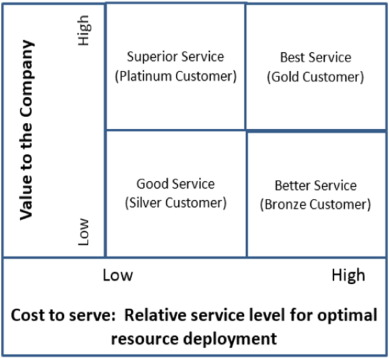
\includegraphics[width=300pt,height=300pt]{./imgs/cpm_matrix} 

}

\caption{CPM Matrix}\label{fig:cpmmat}
\end{figure}

\hypertarget{what-is-attrition}{%
\section{What is attrition?}\label{what-is-attrition}}

Customer \emph{attrition} or churn occurs when a client discontinues using a service or a product offered by a firm. Churn analysis corresponds to measuring the \emph{attrition} rate in the customer base of any company. However, evaluating \emph{attrition} depends on the type of relationship between the firm and its clients. When it is defined by a contract, the customer has to inform the firm about their service termination. In the telecom industry, a consumer is required to notify their telecommunications service provider (TSP) before going to a competing company. In an opposite way, the firm/client relationship can be non-contractual. In that case, the service termination does not need to be notified. \emph{Attrition} then becomes a latent variable and more advanced models are used to make forecasts.

\hypertarget{what-does-customer-value-mean}{%
\section{What does customer ``value'' mean?}\label{what-does-customer-value-mean}}

In \emph{customer portfolio management}, one client's value is represented by the \textbf{customer lifetime value} (CLV). CLV is the present \emph{value} of all future purchases made by a customer over their lifetime in the firm's portfolio, taking into account the \emph{attrition} risk. CLV depends both on the purchase recency as well as on the purchasing rate and aims at identifying the most valuable customer groups. Formally, Gupta and Lehmann \citep{CUSTOMERS_ASSETS} define CLV for customer \(i\) as follows:
\[CLV_i = \sum_{t=0}^{T_i} \frac{(p_t - c_t)r_{i,t}}{(1+a)^t} - AC_i\]

with,

\begin{itemize}
\tightlist
\item
  \(p_t\) the price paid by customer \(i\) at time \(t\)
\item
  \(c_t\) the cost at time \(t\)
\item
  \(r_{i,t}\) the \textbf{probability that customer \(i\) be active} at time \(t\)
\item
  \(a\) the discount rate
\item
  \(AC_i\) the acquisition cost of customer \(i\)
\item
  \(T_i\) the duration of observation
\end{itemize}

An estimation of the portfolio's overall value can be calculated through \textbf{customer equity} (CE) which amounts to the sum of all the CLVs. Since CE appears to be a good proxy of the firm's value, the profit maximization program can be rewritten as:
\[ 
\begin{aligned}
\max_{p} \quad & \textrm{CE} = \sum_{i=1}^{N} \sum_{t=0}^{T_i} \frac{(p_t - c_t)r_{i,t}}{(1+a)^t} - AC_i\\
\textrm{s.t.} \quad & r_{i,t} \in [0, 1]\\
  &p_t > c_t    \\
\end{aligned}
\]

\hypertarget{literature}{%
\chapter{Literature Review}\label{literature}}

\hypertarget{portfolio}{%
\section{On customer portfolio}\label{portfolio}}

\hypertarget{attrition}{%
\section{On attrition}\label{attrition}}

\hypertarget{value}{%
\section{On customer value}\label{value}}

In recent years, \emph{customer portfolio management} (CPM) has focused on optimizing clients' value to the firm. The company's interest lies in knowing how much net benefit it can expect from a customer \emph{today}. These expectations are then used to implement efficient marketing strategies to get the highest return on investment. To that end, two key metrics are estimated by firms, namely customer lifetime value (CLV) and customer equity (CE) (see chapter \ref{definitions} for definitions).

According to Blattberg and Deighton, CLV can be defined as the revenues derived from a customer minus the cost to the firm for maintaining the relationship with the customer over time \citep{CLV_DEF}. As shown by Reinartz and Kumar, CLV modelling depends on the type of relationship a firm has with its clients \citep{CLV_CONTEXT}. In a contractual relationship, customer defections are observed which means that longer lifetime means higher customer value. Conversely, when the relationship is non-contractual, uncertainty arises between the customer's purchase behavior and lifetime.

With the development of data collection tools, companies have lots of customer-level data (or customer transaction data) at their disposal to measure CLV \citep{CLV_NBD}. Consequently, different modelling approaches can be adopted in order to estimate customers' value.

RFM (Recency Frequency Monetary) models are considered the simplest strategy to increase CLV and customer's loyalty \citep{CLV}. It aims at targeting specific marketing campaigns at specific groups of customers to improve response rates. RFM models consists in creating clusters of clients based on three variables:

\begin{itemize}
\tightlist
\item
  \emph{recency} which is the time that has elapsed since a customer's last activity with the firm;
\item
  \emph{frequency} that is the number of times a customer transacted with the brand in a particular period of time;
\item
  \emph{monetary} value of customer's prior purchases.
\end{itemize}

However, RFM models have a limited predictive power since they only predict clients' behavior for the next period.

In their article on CLV management, Borle and Singh draw the review of more advanced modelling techniques that can be implemented to estimate customers' value \citep{CLV_MEASUREMENT}. A popular method to estimate customer lifetime value is the negative binomial distribution (NBD) - Pareto \citep{CLV_NBD} which helps solving the lifetime uncertainty issue. The model takes past customer purchase behavior as input such as the number of purchases in a specific time window and the date of last transaction. Then the model outputs a repurchase probability as well as a transaction forecast for each individual. In Borle and Singh's research paper, a hierarchical bayesian model is implemented with a view to jointly predict customer's churn risk and spending pattern. Here, the main advantage of using a bayesian approach is to give priors on CLV's drivers. The study is base on data coming from a membership-based direct marketing company where firm/client relationships are non-contractual. In other words, the times of each customer joining the membership and terminating it are known once these events happen. Thus the implementation of a sophisticated estimation strategy is justified.

In our study, emphasize is placed on estimating the overall value of a customer portfolio. The methodology we will develop is based on a research paper written by our Econometrics teacher Alain Bousquet, whose goal is provide tools for an efficient management of a patent portfolio \citep{BREVETS}. The main idea is to consider each patent as an asset with a related value which can generate income if this very patent is exploited. This modelling approach can be transposed to customer portfolio analysis with the customer's value corresponding to the CLV and the probability of exploitation being the opposite of the risk of \emph{attrition}. In this context, CLV can be estimated with techniques mentioned above. The client's risk of churn can be modelled with duration models or machine learning techniques as evoked in \ref{attrition}.

\hypertarget{framework}{%
\chapter{Theoretical Framework}\label{framework}}

This chapter presents theoretical basis of the models and the algorithms that are used to model customer portfolios. As a customer's lifetime in a portfolio is usually represented by the time to churn, duration models are adapted to the data we have at our disposal. Thus, it is decided to introduce standard survival techniques as well as machine learning algorithms suited to time-to-event data. Methods to estimate customer's value are also introduced in this chapter.

\hypertarget{duration-models}{%
\section{Duration models}\label{duration-models}}

According to Cameron \& Trivedi \citep{CAMERON_TRIVEDI}, duration models (also called survival models) aims at measuring the time spent in a certain state before transitioning to another state. In Econometrics,

\begin{itemize}
\tightlist
\item
  a \textbf{state} corresponds to the class in which an individual \(i\) is at time \(t\).
\item
  a \textbf{transition} is movement from one state to another.
\item
  a \textbf{duration} measures the time spent in a certain state and is also called a \textbf{spell} length.
\end{itemize}

Since measuring the time until the event is needed for multiple purposes, duration analysis is used in a variety of economic sectors as depicted by the following table.

\begin{longtable}[]{@{}cc@{}}
\toprule
Economic sector & Purpose \\
\midrule
\endhead
Macroeconomics & Length of an unemployment spell \\
Insurance & Risk analysis to offer a segmented pricing \\
Engineering & Time until a device breaks down \\
Epidemiology & Survival time of a virus \\
\textbf{Churn analysis} & \textbf{Time until a customer leave the portfolio} \\
\bottomrule
\end{longtable}

\hypertarget{censoring-and-truncation}{%
\subsection{Censoring and Truncation}\label{censoring-and-truncation}}

When dealing with survival data, some observations are usually \textbf{censored} meaning they are related to spells which are not completely observed. Duration data can also suffer from a selection bias which is called \textbf{truncation}.

\hypertarget{censoring-mechanisms}{%
\subsubsection*{Censoring mechanisms}\label{censoring-mechanisms}}
\addcontentsline{toc}{subsubsection}{Censoring mechanisms}

\textbf{Left-censoring} occurs when the event of interest occurs before the beginning of the observation period. For example, an individual is included in a study of duration of unemployment at \(t_0\). At that time he has already been unemployed for a period but he cannot recall exactly the duration of this period. If we observe that he finds a job again at \(t_1\), we can only deduce that the duration of unemployment is bigger than \(t_1-t_0\), this individual is left-censored. Observation 2 on figure \ref{fig:censoring} is associated with a left-censored spell \citep{LIU_SCOR}.

A spell is considered \textbf{right-censored} when it is observed from time \(t_0\) until a censoring time \(t_c\) as illustrated by observation 1 on figure \ref{fig:censoring}. For instance, the lifetime related to a customer who has not churned at the end of the observation period is right-censored. Let us note \(X_i\) the duration of a complete spell and \(C_i\) the duration of a right-censored spell. We also note \(T_i\) the duration actually observed and \(\delta_i\) the censoring indicator such that \(\delta_i = 0\) if the spell is censored. Then, \((t_1, \delta_1),\dots,(t_N, \delta_N)\) are the realizations of the following random variables:

\begin{equation}
  \begin{aligned}
  T_i & = \min(X_i, C_i) \\
  \delta_i & = \mathbb{1}_{X_i < C_i}
  \end{aligned}
  \label{eq:censoring}
\end{equation}

\hypertarget{selection-bias}{%
\subsubsection*{Selection bias}\label{selection-bias}}
\addcontentsline{toc}{subsubsection}{Selection bias}

Survival data suffers from a \textbf{selection bias} (or truncation) when only a sub-sample of the population of interest is studied. A customer entering the firm's portfolio after the end of the study is said to be \textbf{right-truncated}, whereas a client who has left the portfolio before the beginning of the study is considered \textbf{left-truncated}. Mathematically, a random variable \(X\) is truncated by a subset \(A \in \mathbb{R}^+\) if instead of \(\Omega(X)\), we solely observe \(\Omega(X)\bigcap A\). On figure \ref{fig:censoring}, the first and fifth observations suffers from a selection bias.

\begin{figure}

{\centering 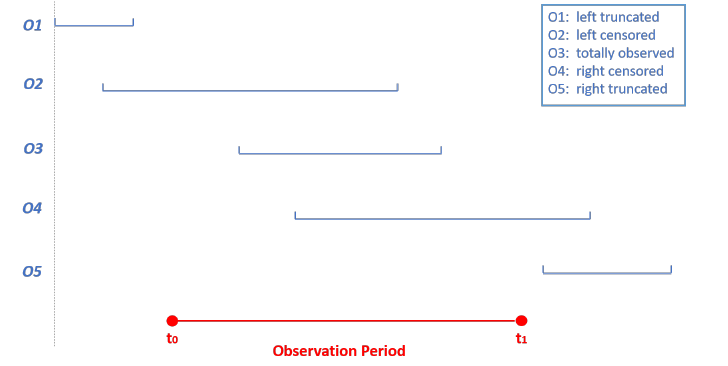
\includegraphics[width=500pt,height=250pt]{./imgs/censoring_and_truncation} 

}

\caption{Censored and truncated data}\label{fig:censoring}
\end{figure}

\hypertarget{probabilistic-concepts}{%
\subsection{Probabilistic concepts}\label{probabilistic-concepts}}

In survival analysis, the response variable denoted \(T\) is a time-to-event variable. Instead of estimating the expected failure time, survival models estimate the \emph{survival} and \emph{hazard rate} functions which depend on the realization of \(T\).

\hypertarget{survival-function}{%
\subsubsection*{Survival function}\label{survival-function}}
\addcontentsline{toc}{subsubsection}{Survival function}

The survival function \(S(t)\) represents the probability that the considered event occurs after time \(t\). For instance, \(S(t)\) can measure the probability that a given customer survive in the portfolio at least until time \(t\). Mathematically, the survival function is defined as:
\begin{equation}
  S(t) = P(T > t) = 1 - F(t)
  \label{eq:survfun}
\end{equation}

where \(F(t)\) is the cumulative distribution function.

\begin{figure}

{\centering 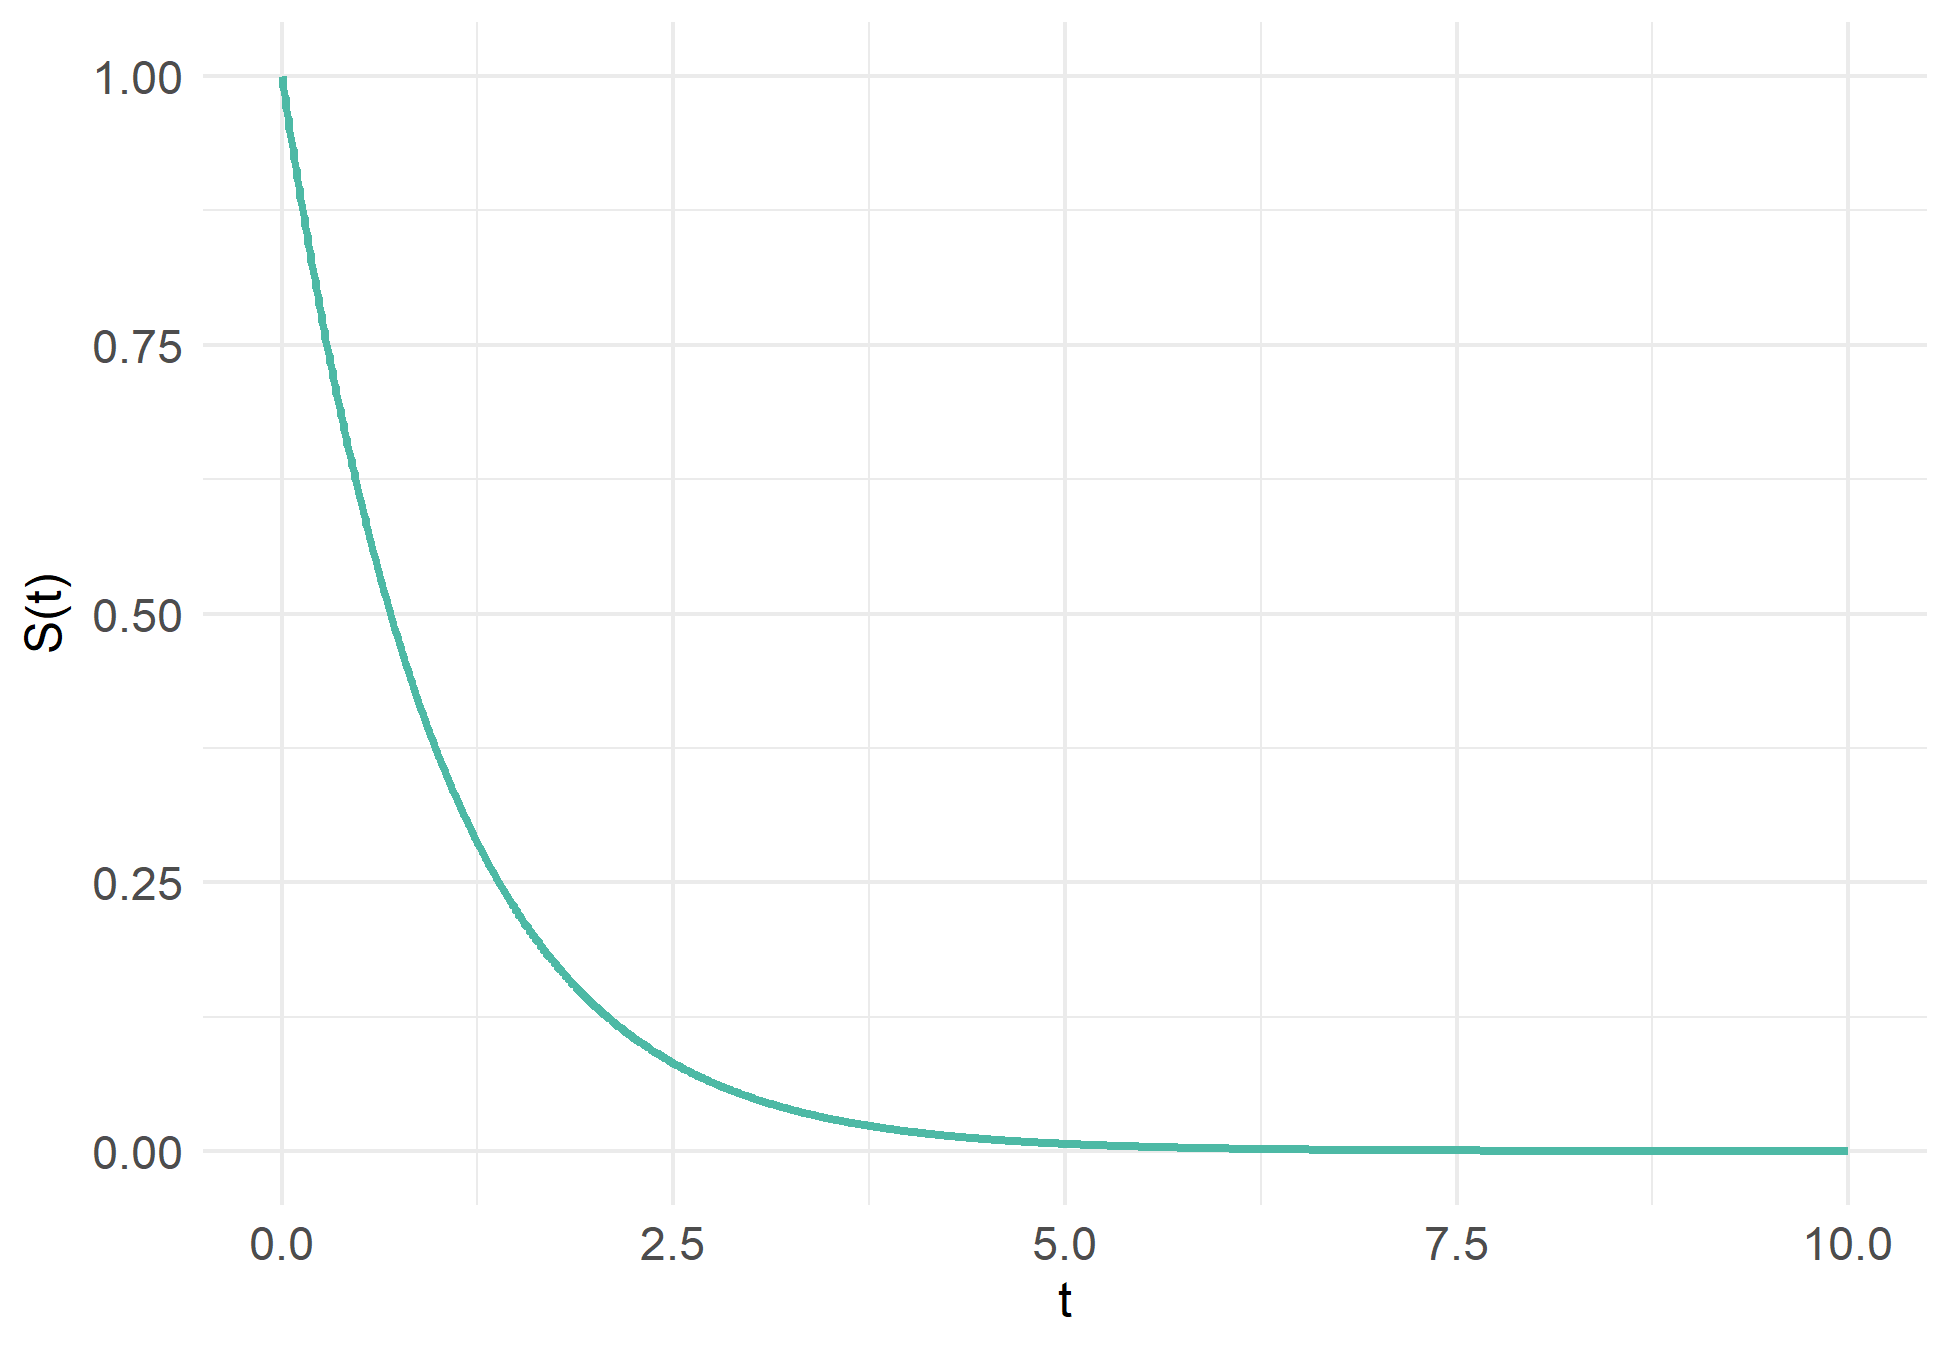
\includegraphics[width=400pt,height=300pt]{./imgs/surv_fun_plot} 

}

\caption{Survival function $S_T(t)$ with $T \sim \mathcal{E} (1)$}\label{fig:survfunplot}
\end{figure}

\hypertarget{hazard-and-cumulative-hazard-functions}{%
\subsubsection*{Hazard and Cumulative Hazard functions}\label{hazard-and-cumulative-hazard-functions}}
\addcontentsline{toc}{subsubsection}{Hazard and Cumulative Hazard functions}

Another key concept in duration analysis is the hazard function \(\lambda(t)\) which approximates the probability that the event occurs at time \(t\). For instance, \(\lambda(t)\) can measure the probability that a given individual leaves the firm portfolio at time \(t\). Formally, it is expressed as follows:
\begin{equation}
  \lambda(t) = \lim_{\Delta t \to 0} \frac{P\big[t \leq T < t + \Delta t | T \geq t \big]}{\Delta t}
  \label{eq:hazfun}
\end{equation}

Using the Bayes formula, equation \eqref{eq:hazfun} can also be written as (see equation \eqref{eq:hazfunproof} in appendix):
\begin{equation}
  \lambda(t) = \frac{-\text{d} \ln \big(S(t)\big)}{\text{d} t}
  \label{eq:hazfunbis}
\end{equation}

Finally, integrating the instantaneous hazard function gives the cumulative hazard function which can be more precisely estimated than the hazard function \citep{CAMERON_TRIVEDI} and is defined as:

\begin{equation}
  \Lambda (t) = \int_{0}^{t} \lambda(s) \text{d}s = \ln \big(S(t)\big)
  \label{eq:cumhazfun}
\end{equation}

\begin{figure}

{\centering 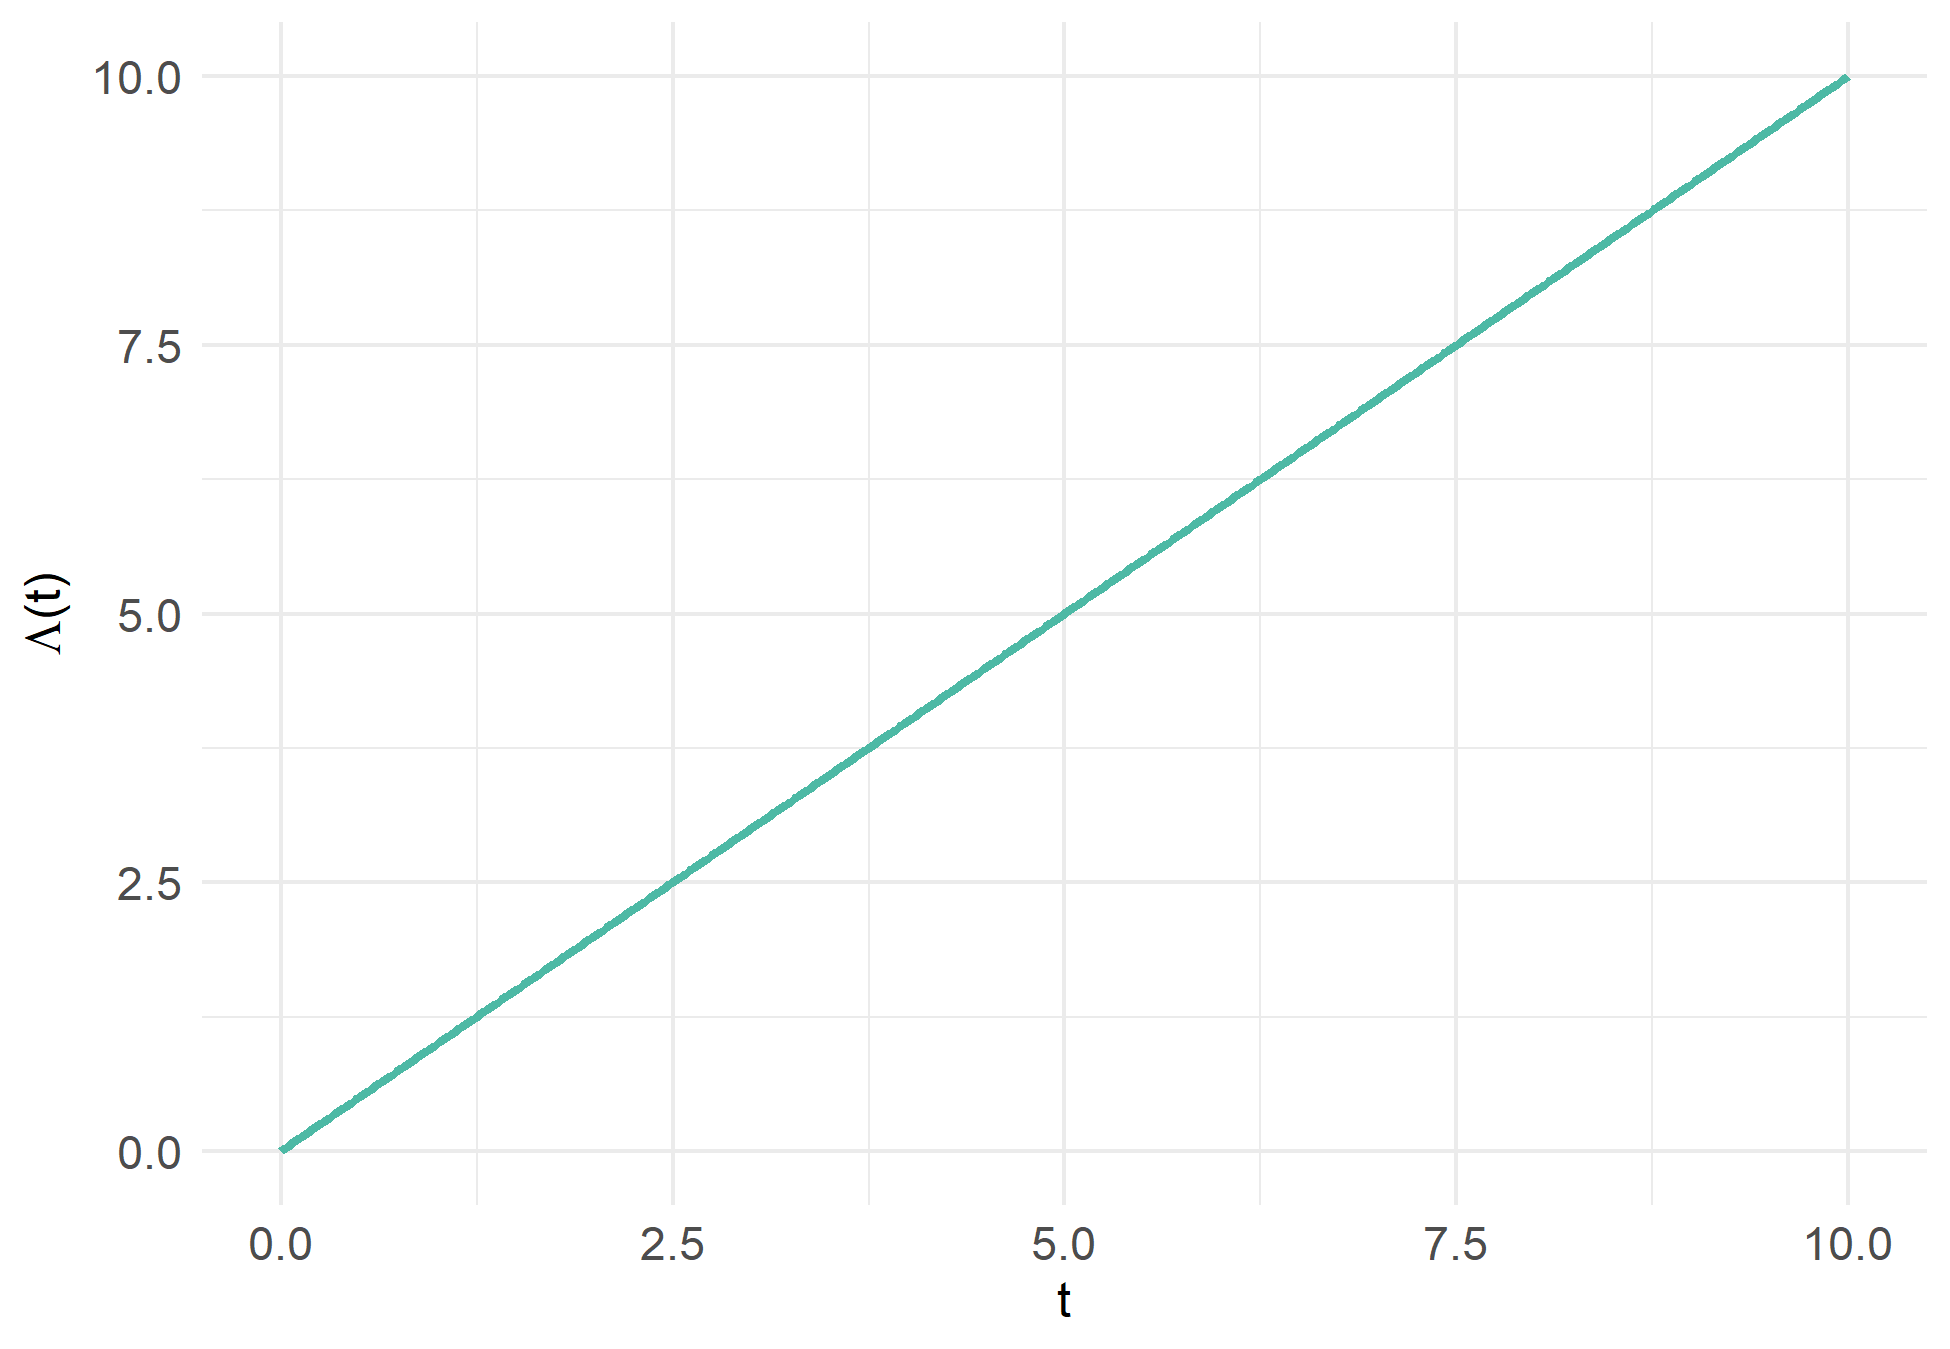
\includegraphics[width=400pt,height=300pt]{./imgs/cum_haz_plot} 

}

\caption{Cumulative Hazard function $\Lambda_T(t)$ with $T \sim \mathcal{E} (1)$}\label{fig:cumhazplot}
\end{figure}

Thus, the hazard, survival and cumulative hazard functions are three mathematical functions which describe the same distribution.

\hypertarget{nonparametric-models}{%
\subsection{Nonparametric models}\label{nonparametric-models}}

When dealing with duration data, these methods are helpful to have a general overview of the raw (unconditional) hazard. Nonparametric models are rather used for data description rather than prediction. No explanatory variable is included in these models except for treatment variables such as the type of contract a customer has subscribe.

\hypertarget{notations}{%
\subsubsection*{Notations}\label{notations}}
\addcontentsline{toc}{subsubsection}{Notations}

Let us consider a sample with \(N\) observations with \(k\) discrete failure time (e.g.~a failure can be a churn event), such that \(\forall j \in [\![1; k]\!]\) :

\begin{itemize}
\tightlist
\item
  \(t_j\) the \(j^{\text{th}}\) discrete failure time,
\item
  \(d_j\) the number of spells terminating at \(t_j\),
\item
  \(m_j\) the number of right-censored spells in the interval \([t_j, t_{j+1}]\),
\item
  \(r_j\) the number of exposed durations right before time \(t_j\) such that:
  \begin{equation}
  r_j = (d_j + m_j) + \dots + (d_k + m_k) = \sum_{l|l \geq j} (d_l + m_l)
  \label{eq:exposed}
  \end{equation}
\end{itemize}

\hypertarget{hazard-function-estimator}{%
\subsubsection*{Hazard function estimator}\label{hazard-function-estimator}}
\addcontentsline{toc}{subsubsection}{Hazard function estimator}

As the instantaneous hazard at time \(t_j\) is defined as \(\lambda_j = P[T=t_j|T\geq t_j]\), a trivial estimator of \(\lambda_j\) is obtained by dividing the number of durations for which the event is realized in \(t_j\) by the total number of exposed durations at time \(t_j^{-}\). Formally, it is expressed as:

\begin{equation}
  \hat{\lambda}_j = \frac{d_j}{r_j}
  \label{eq:hazest}
\end{equation}

\hypertarget{kaplan-meier-estimator}{%
\subsubsection*{Kaplan-Meier estimator}\label{kaplan-meier-estimator}}
\addcontentsline{toc}{subsubsection}{Kaplan-Meier estimator}

Once the hazard function estimator computed, the discrete-time survivor function can be estimated using the Kaplan-Meier product-limit estimator. To estimate the survival at time \(t\), this estimator computes the joint probability that a spell stays in the same state until \(t\) (e.g.~remaining loyal to a firm until a certain time). This method is based on conditional probabilities and the survival function estimate is defined as:

\begin{equation}
  \hat{S}(t) = \Pi_{j|t_j \leq t} \big(1-\hat{\lambda}_j\big) = \Pi_{j|t_j \leq t}\frac{r_j - d_j}{r_j}
  \label{eq:kaplanmeier}
\end{equation}

When plotting the survival curve after having performed the Kaplan-Meier estimation, confidence bands are also added to the plot in order to reflect sampling variability \citep{CAMERON_TRIVEDI}. The confidence interval of the survival function \(S(t)\) is derived from the estimate of the variance of \(S(t)\) which is obtained by the Grenwood estimate (see equation \eqref{eq:greenwood}).

\begin{equation}
  \hat{\mathrm{V}}[\hat{S}(t)] = \hat{S}(t)^2 \sum_{j|t_j \leq t} \frac{d_j}{r_j(r_j-d_j)}
  \label{eq:greenwood}
\end{equation}

\hypertarget{nelson-aalen-estimator}{%
\subsubsection*{Nelson-Aalen estimator}\label{nelson-aalen-estimator}}
\addcontentsline{toc}{subsubsection}{Nelson-Aalen estimator}

The cumulative hazard function estimate is given by the Nelson-Aalen estimator which consists in summing up the hazard estimates for each failure time.

\begin{equation}
  \hat{\Lambda}(t) = \sum_{j | t_j \leq t} \hat{\lambda}_{j} = \sum_{j | t_j \leq t} \frac{d_j}{r_j}
  \label{eq:nelsonaalen}
\end{equation}

Exponentiating \(\hat{\Lambda}(t)\), one can obtain a second estimate of the survival function (see equation \eqref{eq:linksurvcumhaz} in the appendix):

\begin{equation}
    \tilde{S}(t) = \exp \big( -\hat{\Lambda}(t) \big)
    \label{eq:survest}
\end{equation}

\hypertarget{parametric-models}{%
\subsection{Parametric models}\label{parametric-models}}

The nonparametric estimation is undoubtedly useful when it comes to have a general overview on the survival data. However, one may want to model the hazard and survivor functions with a functional form in which unknown parameters need to be optimized. In parametric estimation, there are two main groups of models to estimate the conditional hazard function \(\lambda(t | \pmb{x})\):

\begin{itemize}
\tightlist
\item
  the Parametric Proportional Hazards (AFT) models,
\item
  the Accelerated Failure Time models (PH).
\end{itemize}

When implementing parametric models, \(\lambda\), \(S\) and \(\Lambda\) are expressed based on the chosen parametric form. The instantaneous hazard function can either be constant or monotone.

\hypertarget{ML}{%
\section{Machine Learning techniques}\label{ML}}

\hypertarget{data}{%
\chapter{Data}\label{data}}

\hypertarget{appendix}{%
\chapter*{Appendix}\label{appendix}}
\addcontentsline{toc}{chapter}{Appendix}

In this part, some proofs of the mathematical concepts used in the study are derived.

\hypertarget{duration-models-1}{%
\section*{Duration models}\label{duration-models-1}}
\addcontentsline{toc}{section}{Duration models}

\textbf{Hazard function}

\begin{equation}    
  \begin{aligned}
  \lambda(t) & = \lim_{\Delta t \to 0} \frac{P\big[t \leq T < t + \Delta t | T \geq t \big]}{\Delta t} \\\\
  & = \lim_{\Delta t \to 0} \frac{P\big[t \leq T < t + \Delta t \big] / P\big[T \geq t  \big]}{\Delta t} \\\\
  & = \lim_{\Delta t \to 0} \frac{\big(F(t+\Delta t)-F(t)\big) / \Delta t}{S(t)} \\\\
  & = \frac{\text{d} F(t) / \text{d} t}{S(t)} \\\\
  & = \frac{f(t)}{S(t)} \\\\
  \lambda(t) & = \frac{-\text{d} \ln \big(S(t)\big)}{\text{d} t}
  \end{aligned}
  \label{eq:hazfunproof}
\end{equation}

\textbf{Link between cumulative hazard and survivor functions}

\begin{equation}
  \begin{aligned}
  \Lambda(t)      & = \int_{0}^{t} \lambda(s)ds \\\\
  \iff \Lambda(t) & = \int_{0}^{t} \frac{f(s)}{S(s)}ds \\\\
  \iff \Lambda(t) & = -\ln \big(S(t)\big) \\\\
  \iff S(t)       & = \exp \big(-\Lambda(t)\big)
  \end{aligned}
  \label{eq:linksurvcumhaz}
\end{equation}

  \bibliography{biblio.bib,packages.bib}

\end{document}
